\chapter{Apache Cassandra}
\chapterauthor{David Marchi, Daniel Schäfer, Erik Zeiske}

\section{Introduction}
    %- History, relevance, environment, context
    %- Task, goal, why, what
    %- Structure
% Evaluationg NOSQL Databases under the scope of cap=theorem


The following chapter aims to bring an overview into the Cassandra data store as well as detailed information about how it works and its architecture.
After that, a detailed guide on how to model data for Cassandra in order to make the best use out of the architecture will follow.
Transitioning into technical details and examples on how Cassandra works, what features and pitfalls it brings with it.


Many large companies and organizations have deployed Cassandra clusters.
Here is an overview of exceptional cases: \\

 \begin{tabular}{@{}ll}
   \gls{cern}    & Storage backend for \gls{atlas} detector \autocite{cassandra_cern} \\
   \hline
   Netflix & 2,500 nodes, 420 TB, over 1 trillion requests per day \\
           & Migrated from Oracle to Cassandra \autocite{cassandra_netflix} \\
   \hline
   eBay    & 6 billion writes and 5 billion reads daily \\
           & Single Cassandra table of 40TB \autocite{cassandra_ebay, cassandra_ebay2} \\
   \hline
   Apple   & More than 75k Cassandra nodes with 10PB in production \\
           & Several clusters with 1000+ nodes each \autocite{cassandra_apple} \\
 \end{tabular}

This shows that Cassandra is heavily used in large-scale deployments of big tech companies and other organizations. The significance of Cassandra and the problems it solves is, with an ever growing amount of data, high.
For trying out Cassandra on a single node or a small local cluster however all of those settings can be left at their defaults. To keep this chapter at a manageable size we will not explain the topological features, only mention which are available.
This chapter will be wrapped up with instructions and hints for trying out Cassandra on a single node or a small local cluster.
Cassandra can be made aware of the relative physical location of all nodes, for example in which rack or data center they are. For real world usage it is recommended to do that and also adjust the configuration to take that into account.

\subsection{Overview of Cassandra}
Cassandra is a Wide Column Store Database. It is table-like but not relational. The architecture and design make it a distributed and masterless data store for large data. It is written in Java and can be run distributed on commodity hardware. Since it is masterless there is no single point of failure. Nodes (connected instances running Cassandra) can be hot-swapped or be temporarily down without affecting the availability of the Cassandra cluster. Adding a new node and removing one will elastically increase or decrease the cluster size without any major impact on the distributed system. This can be refereed to as elastic scalability. All these features make Cassandra highly available and fault tolerance. Depending on the settings, a cluster of Cassandra nodes can be more or less consistent. From eventually consistent, the lowest setting for consistency, to highly consistent. This can be referred to as tunable consistency and allows for a configuration dependent classification in the CAP Theorem. More on that in section~\ref{sec:CassandraClusterArchitecture}.

Cassandra was originally developed by Facebook in 2008, the co-author of Amazons DynamoDB was involved in the development process. Hence Cassandra shares similarities with the architecture of DynamoDB \autocite{cassandra_paper}.
Currently (Apr/19) it is a free software project of the Apache Foundation. Development is mainly driven by DataStax. A company designated for commercial Cassandra use and enterprise support.

\section{Wide Column Store}

A wide column store is a tabular but not relational approach to store data. It is not column oriented, since the rows are stored together. A row can have missing columns which are not stored on disk. This makes it sparse.
It can be thought of like a key-value store where the value can have a subset of a predefined set of columns. Or, put in other words; "Sparse, distributed multi-dimensional sorted map" \autocite{chang2008bigtable}
The naming can be explained as a key value store with wide (complex) values that consist of columns.

\begin{figure}[H]
    \centering
    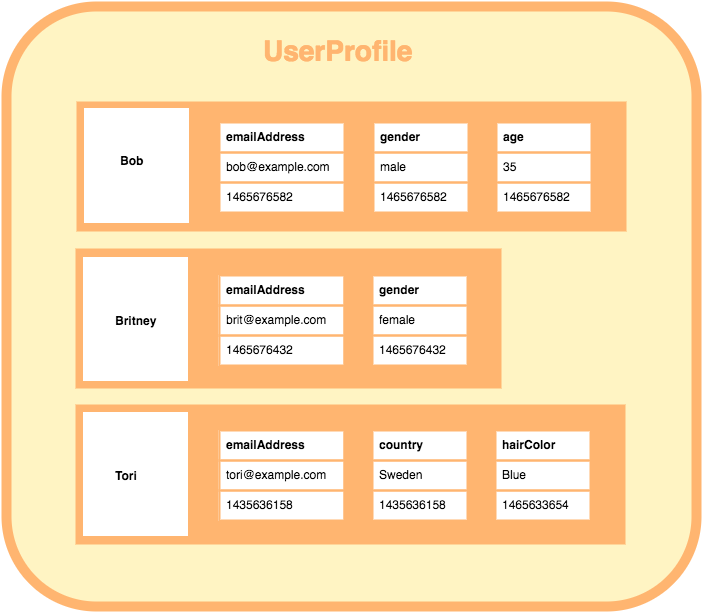
\includegraphics[width=0.75\columnwidth]{img/wide_column_store.png}
    \caption{Example entity relation model \autocite{wideColumnGraphic}}
    \label{fig:cassandra:wide_column}
\end{figure}

\ref{fig:cassandra:wide_column} shows in a graphical representation the structure of a wide column store. The name is the primary key and different people have different columns. The columns with no data are not stored as null but rather not even stored as a whole.

\section{Use-Cases Cassandra}
Cassandra comes with strong benefits over other database systems. These benefits and extra features make it miss some features which one might expect as standard in database systems.
It should be carefully considered whether to use Cassandra or not since it is not the jack of all trades.
One benefit of Cassandra is fast writes which means it can handle a high throughput but the latency might not be too short. These writes include the operations of {INSERT}, {UPDATE} and {DELETE}.
The way Cassandra handles those operations make them equal to a "regular" write operation. This will be explained in section \ref{sec:cassandra:cql}. Another key benefit is high availability. Due to its architecture and depending on the settings, a Cassandra setup can be highly available. Since one of the base assumptions of a distributed system is the expensiveness of inter-node communication, it has an linear horizontal scalability.
The communication between nodes does not increase with the size of node. Due to its distributed nature, the architecture does not rely on a master-slave setting and comes masterless.
Furthermore it can be configured to work with several clusters, globally distributed, which makes for example multicloud Cassandra setups possible.
This means that any client can read from and write to any node. As described previously Cassandra is a wide column store database which results in having a flexible schema where rows can have missing columns that are not stored on disk.
Cassandra has its own query language which is similar \gls{sql} and called \gls{cql}. This makes it easier to use Cassandra if knowledge from \gls{sql} is available.

If any of these points apply to a project or Use-Case, Cassandra is probably a good fit.
But to be sure it is even more important to rule out the cases where Cassandra is not a good fit.
The following paragraph will describe limits of Cassandra. If the use-case needs any of those features, Cassandra will most likely not suffice to fulfill requirements.
First, a single system instance with Cassandra should be avoided. Most of the features and benefits come with multiple node setups. Use-Cases which would need a dozen nodes seem to find a great fit with the distributed storage system.

Equally important is the way data has to be stored and accessed. Due to its architecture, data has to be modeled different in Cassandra. \acrshort{acid} transactions are not possible and tables are fine-tuned for pre defined queries. Those queries should be known early on and not change during use. It is not easily possible to change or extent those queries. Furthermore there are no relations between tables. It is possible to link, connect and reuse IDs but this has to be handled on client side, there are no operations on those IDs available. Additionally column aggregation operations such as \texttt{GROUP BY} are also not possible, since such operations would be very inefficient in a distributed wide column storage.

Having a lot of updates and deletes interspersed with reads slow the system down due to the way of handling requests - just appending data, not changing records and merging them while reading. This has affects on data validation as well. It is not possible to check on write for data uniqueness, constraints or auto increments. \autocite{cassandra_oreilly}

To sum it up there are general Use-Case conditions where Cassandra is a great fit.
In order to make an educated decision the following key-points should fit with the Use-Case and environment:

\begin{itemize}
    \item Large Deployments
    \item High write throughput
    \begin{itemize}
      \item{"High performance at high write volumes with many concurrent client threads"} \autocite{cassandra_oreilly}
    \end{itemize}
    \item Geographical distribution of data and database clients
    \item Different columns per row
\end{itemize}


\section{Data Modeling in Cassandra}  % How to model data (or rather tables)

Compared to other database systems like traditional relational database systems, data modeling is different in Cassandra. Here is a little example to understand the different way of thinking when modeling data for Cassandras wide column data store. \\

Figure~\ref{fig:cassandra:model_data0} shows an example entity relationship diagram of data in the context of a hotel environment. The hotel has the attributes \textit{address}, \textit{phone}, \textit{name} and an \textit{id} as unique primary key. Each hotel has certain amounts of rooms which store information them-self and are connected to other entities.

\begin{figure}[H]
    \centering
    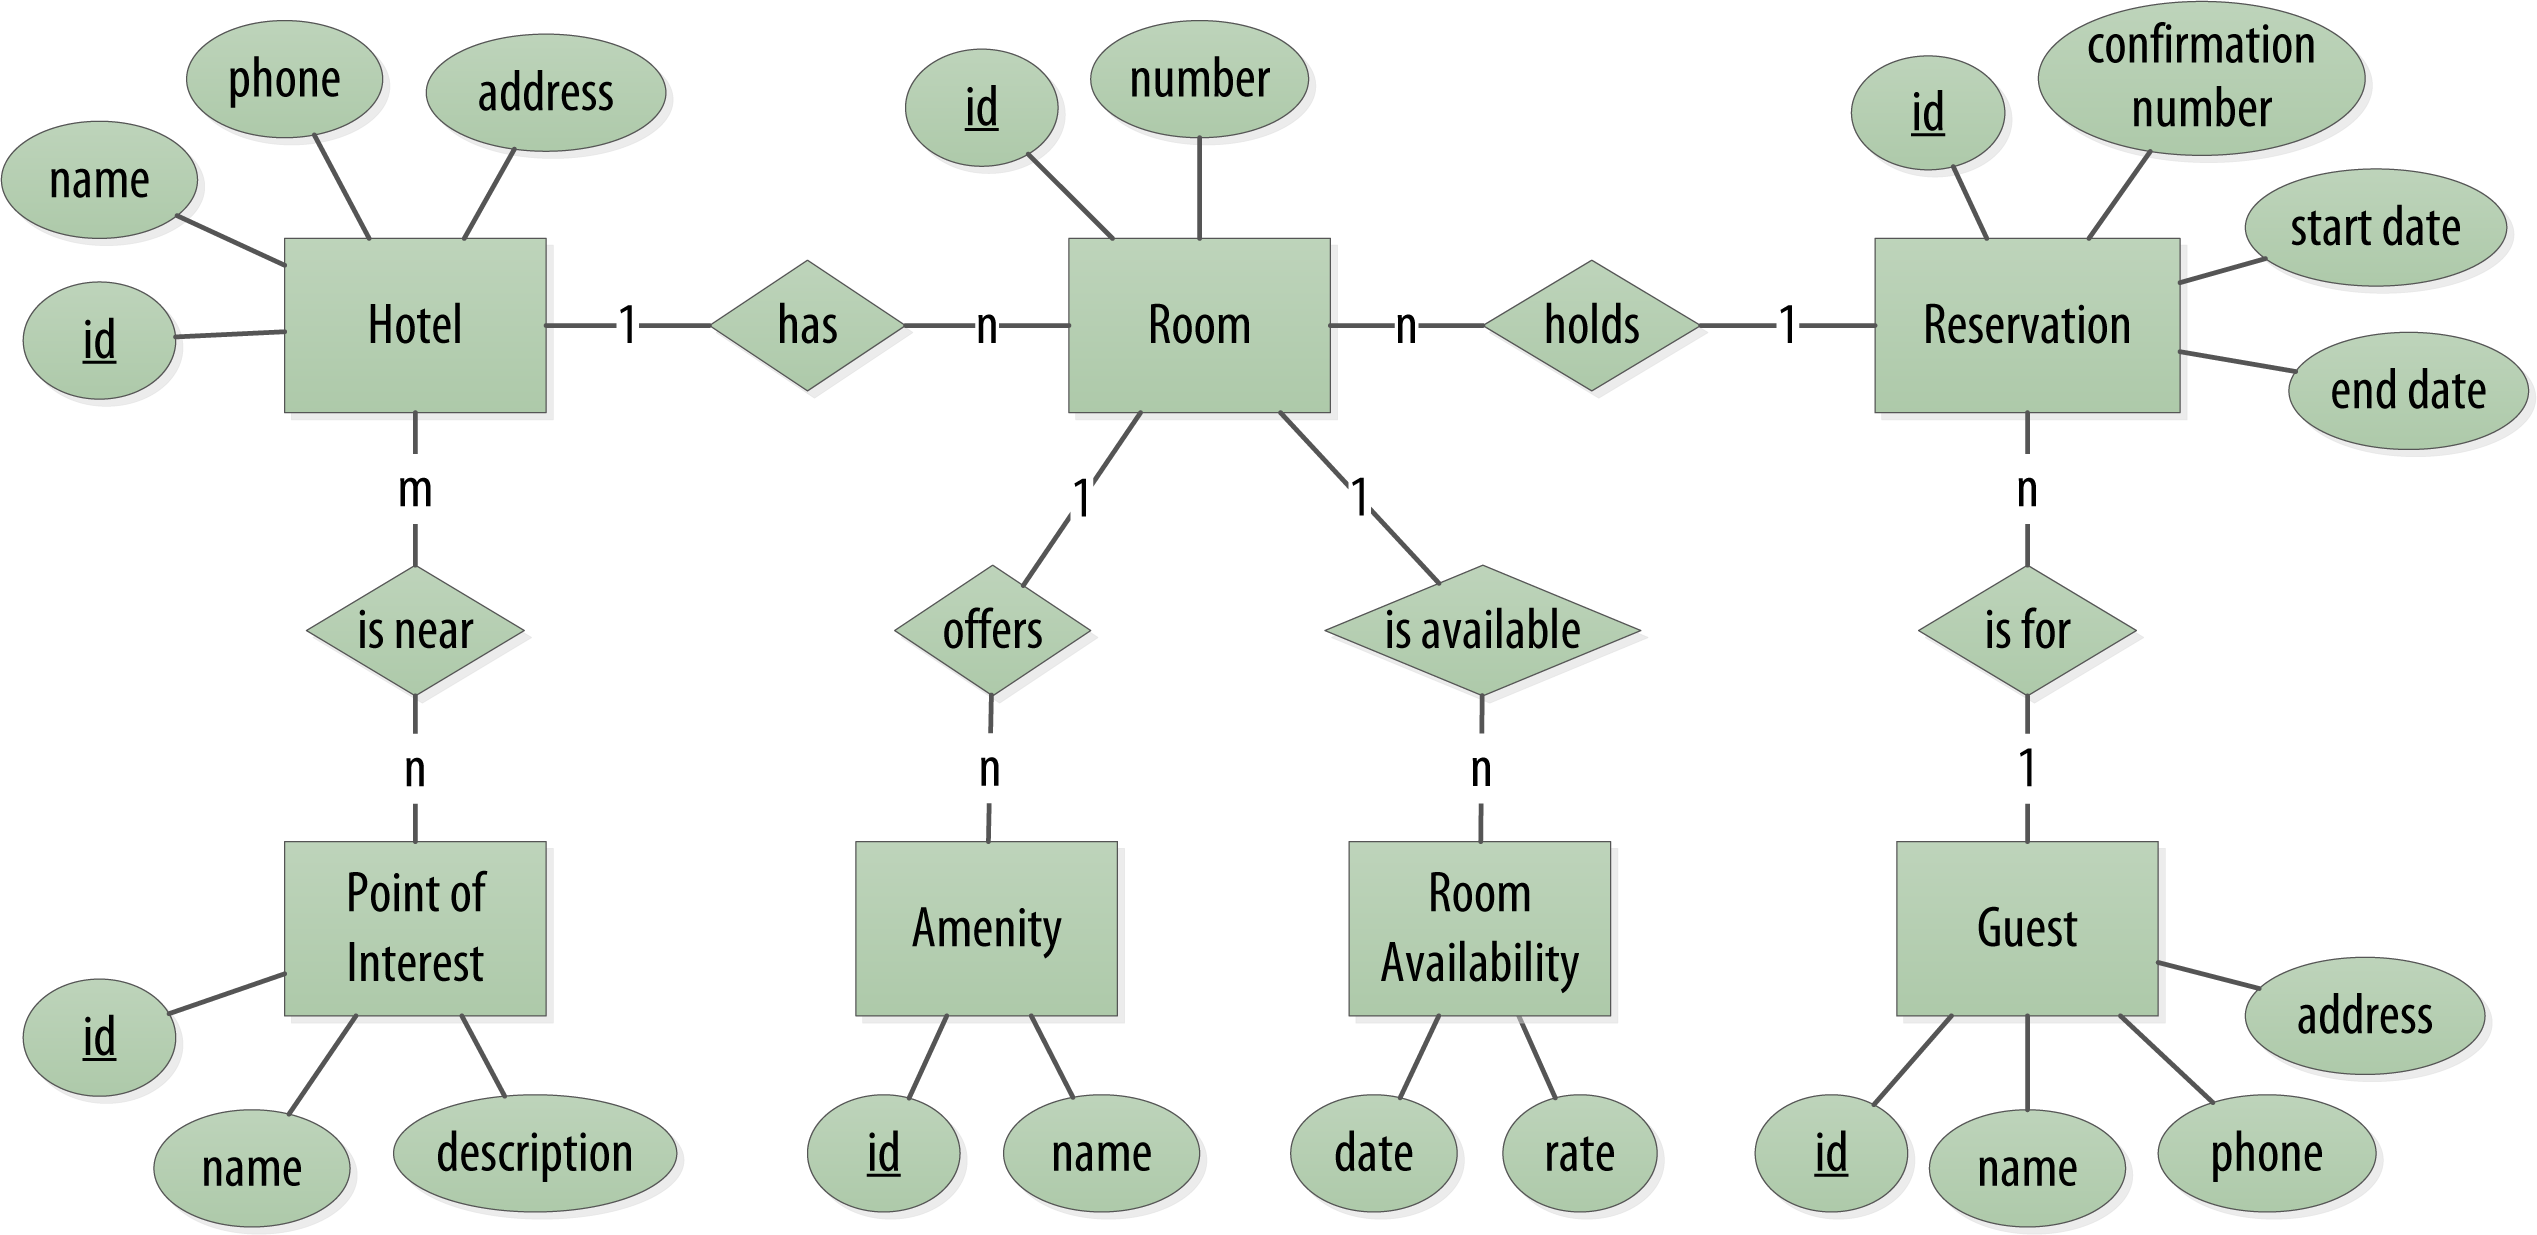
\includegraphics[width=0.75\columnwidth]{img/model_example_entity_relation_step0.png}
    \caption{Example entity relation model \autocite{cassandra_oreilly}}
    \label{fig:cassandra:model_data0}
\end{figure}

In figure~\ref{fig:cassandra:model_data1} an example database model for an relational database of the ERP from figure~\ref{fig:cassandra:model_data0}.
The connections and primary keys previously noted connect now the table to enable complex join queries over multiple tables later on.

\begin{figure}[H]
    \centering
    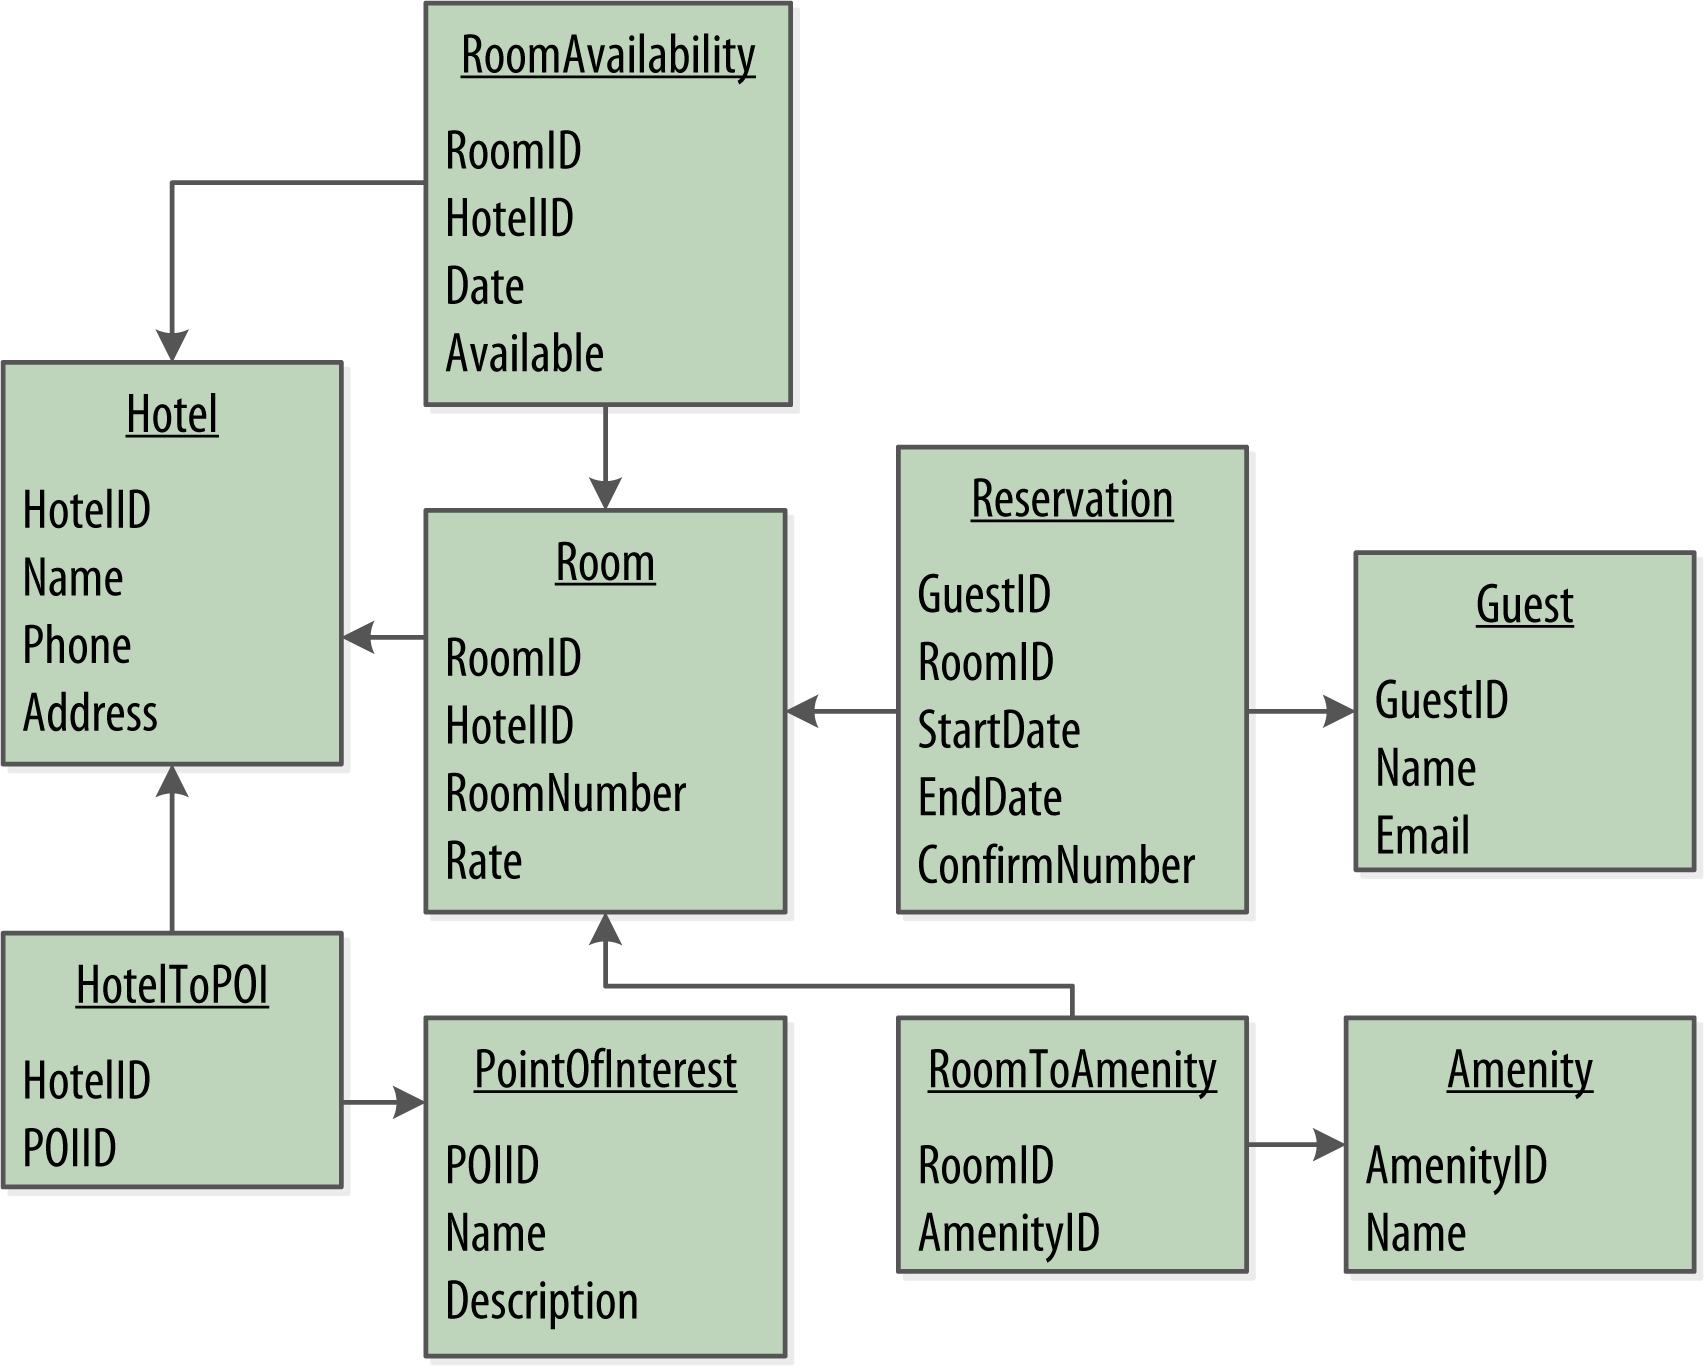
\includegraphics[width=0.75\columnwidth]{img/model_example_rdbms_step1.png}
    \caption{Example RDMBS normalization transition \autocite{cassandra_oreilly}}
    \label{fig:cassandra:model_data1}
\end{figure}

The fundamental difference between those two modeling types is the starting point. In the example above it was all about what data has to be stored and how that data is connected to each other.
In data modeling for Cassandra the queries are the starting points. This means for the architect that they first have to think about queries the database system has to answer.

\begin{figure}[H]
    \centering
    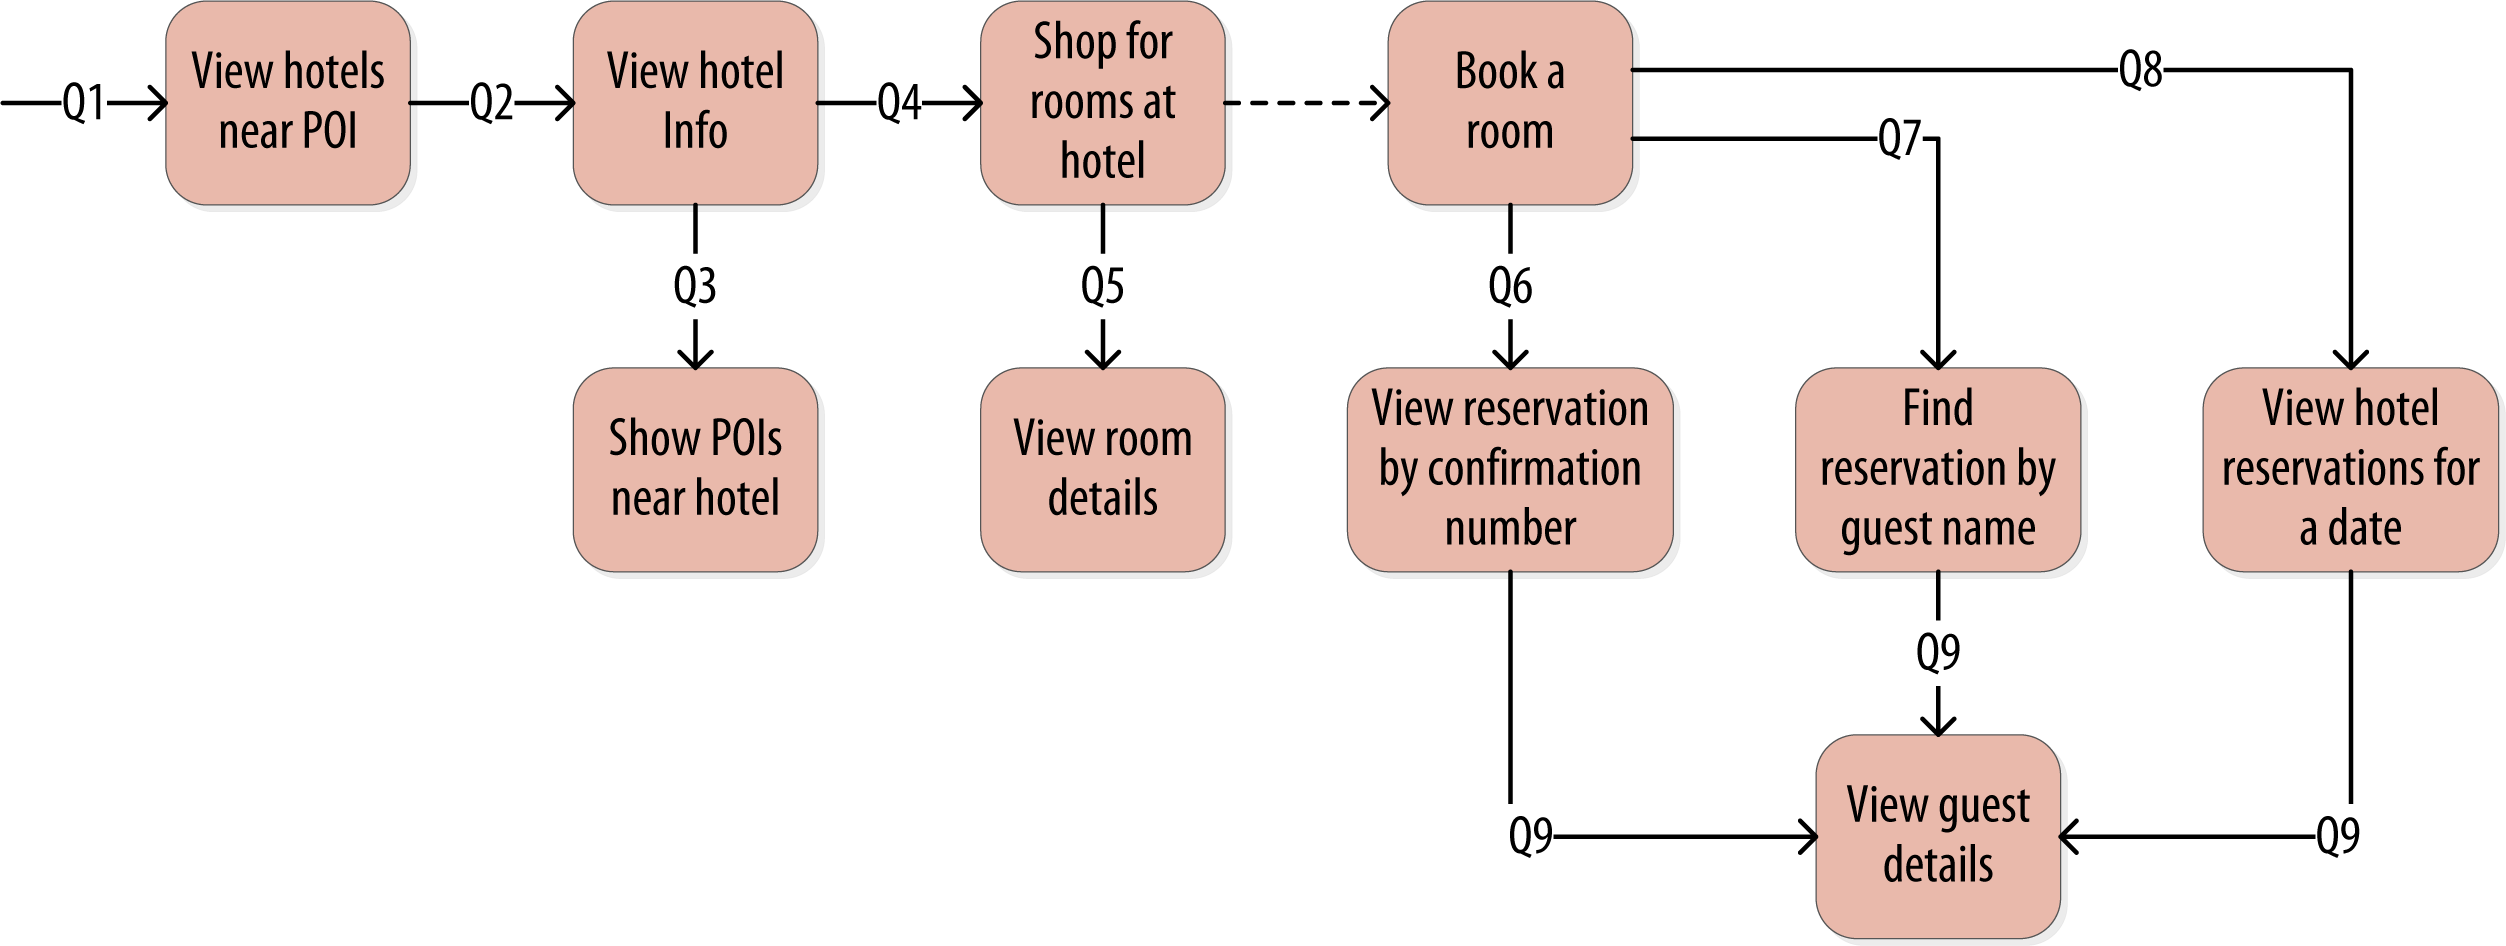
\includegraphics[width=0.75\columnwidth]{img/model_example_queries_step2.png}
    \caption{Planned queries against database system \autocite{cassandra_oreilly}}
    \label{fig:cassandra:model_data2}
\end{figure}

Figure~\ref{fig:cassandra:model_data2} show this circumstance; queries the system later has to answer to. This diagram describes a classical use-case for the hotel environment in which the database would come to work. A user searches for hotels, checks information about it and reserves it.

\begin{figure}[H]
    \centering
    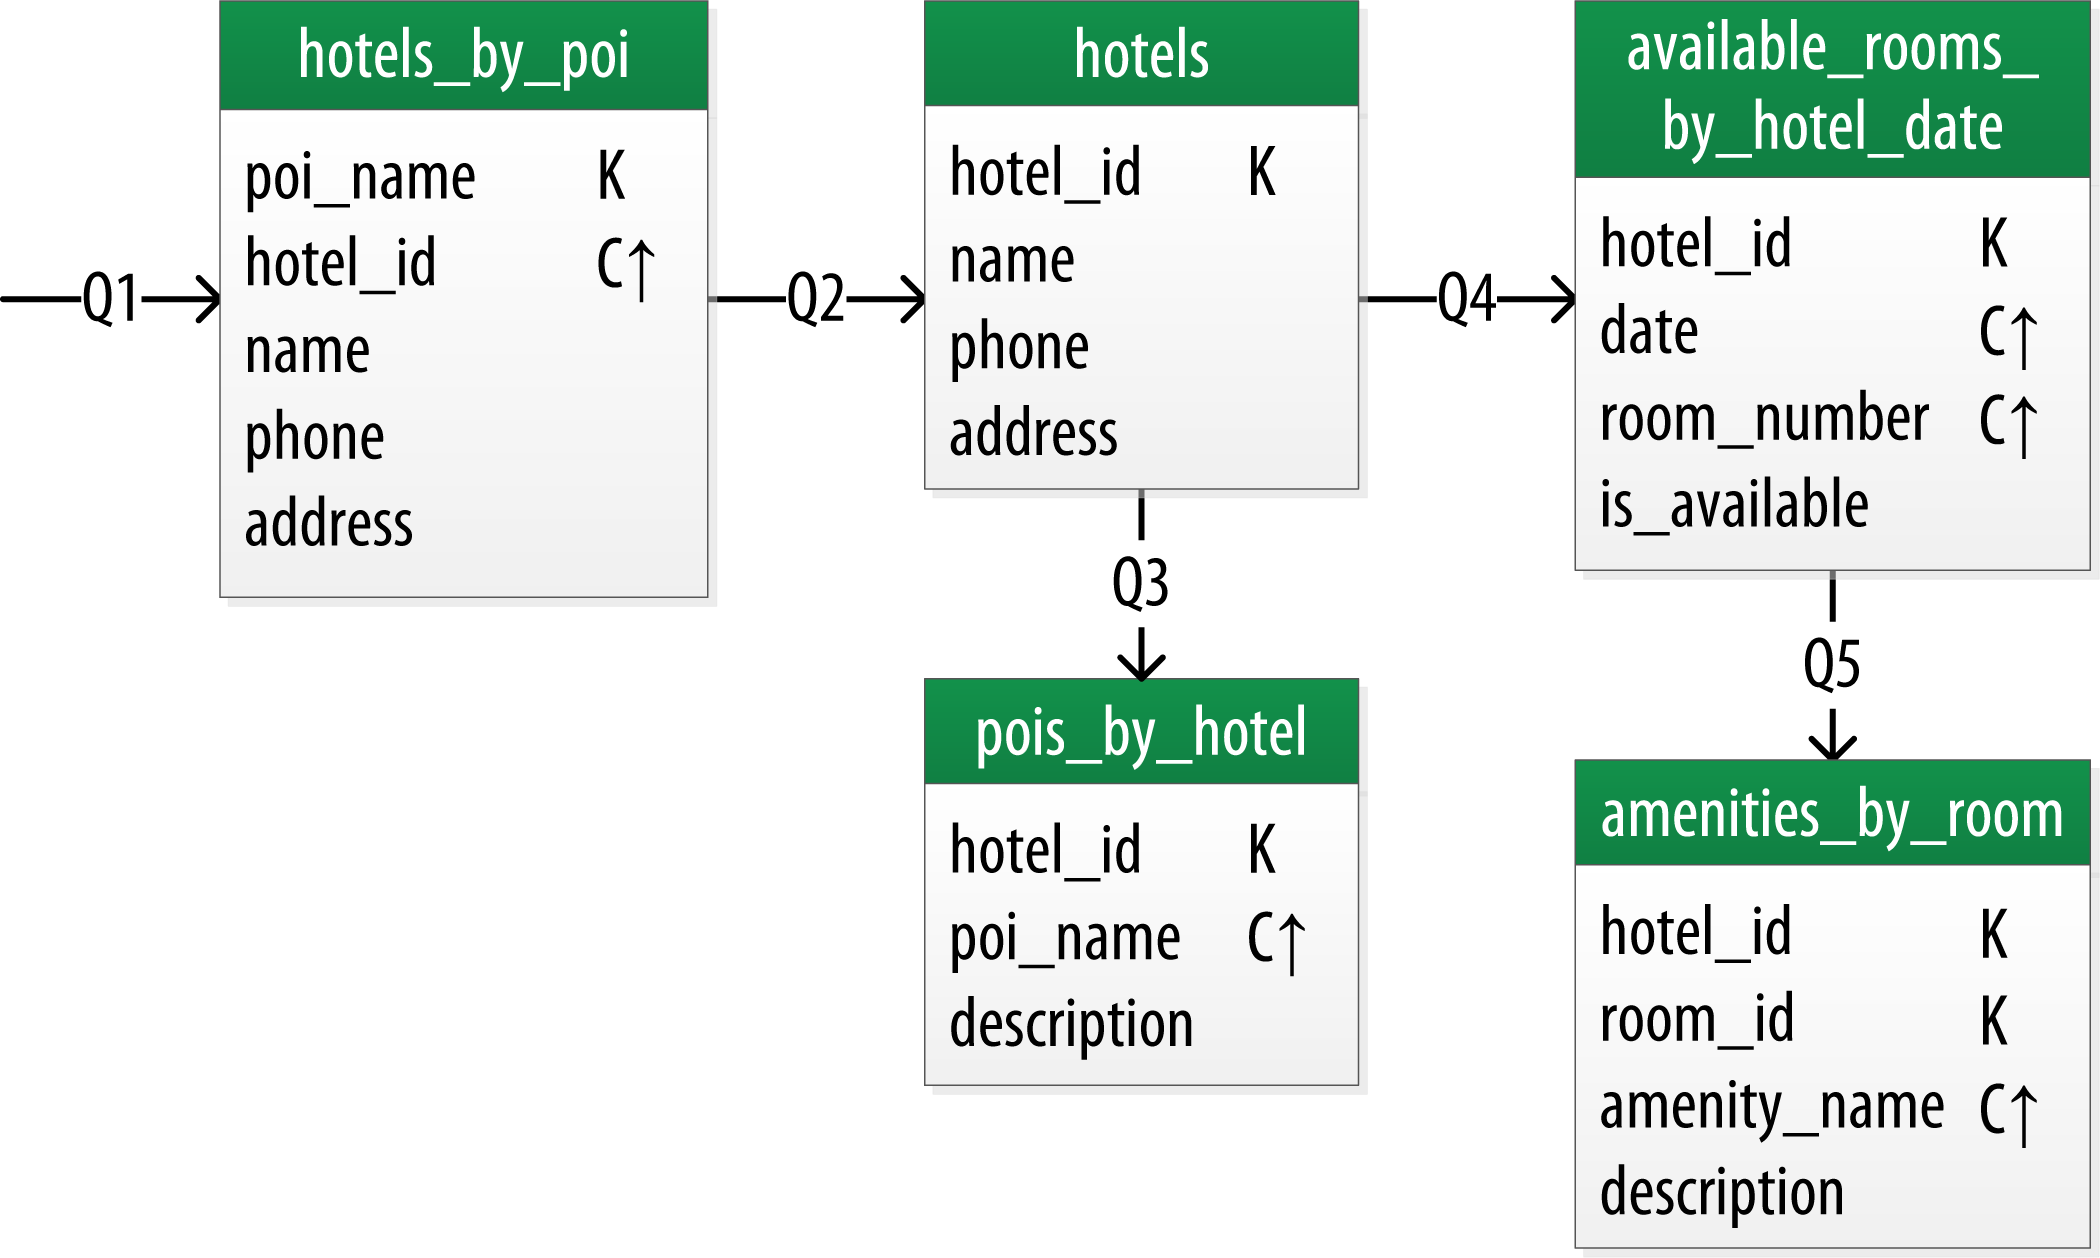
\includegraphics[width=0.75\columnwidth]{img/model_example_chebotko_step3.png}
    \caption{Model and denormalize tables to fit queries \autocite{cassandra_oreilly}}
    \label{fig:cassandra:model_data3}
\end{figure}

Transitioning from the collection of queries in figure~\ref{fig:cassandra:model_data2} to accessible tables, can be seen in figure~\ref{fig:cassandra:model_data3}. It can be seen that data is stored redundantly, available on multiple tables. This does not bother the modeling since queries later on will not use any sort of join operation and be limited onto one table request - which is precisely why data is stored in multiple tables. Each table fulfills one of the queries previously thought of. Furthermore since there is no referential integrity it is possible to store \textit{ids} in tables but the database system does not provide any functionality to make use of and / or connect those \textit{ids}.

In order to properly graph and document this type of modeling, a uniform and new way was proposed to write down data modeling for Cassandra and other similar systems with same needs. \autocite{chebotko2015data}
These diagrams are called Chebotko diagrams and include the way queries are planned. This can be seen in figure~\ref{fig:cassandra:model_data2}.
Out of this table, the diagram can be concluded. Creating to each query an unique table with all necessary information. The arrows with the queries numbers (Q1, Q2 ..) will be kept to keep the context and relation to the previous diagram (\ref{fig:cassandra:model_data3}).
This can be seen in a descriptive example section around figure~\ref{fig:cassandra:chebotko}

\begin{figure}[H]
    \centering
    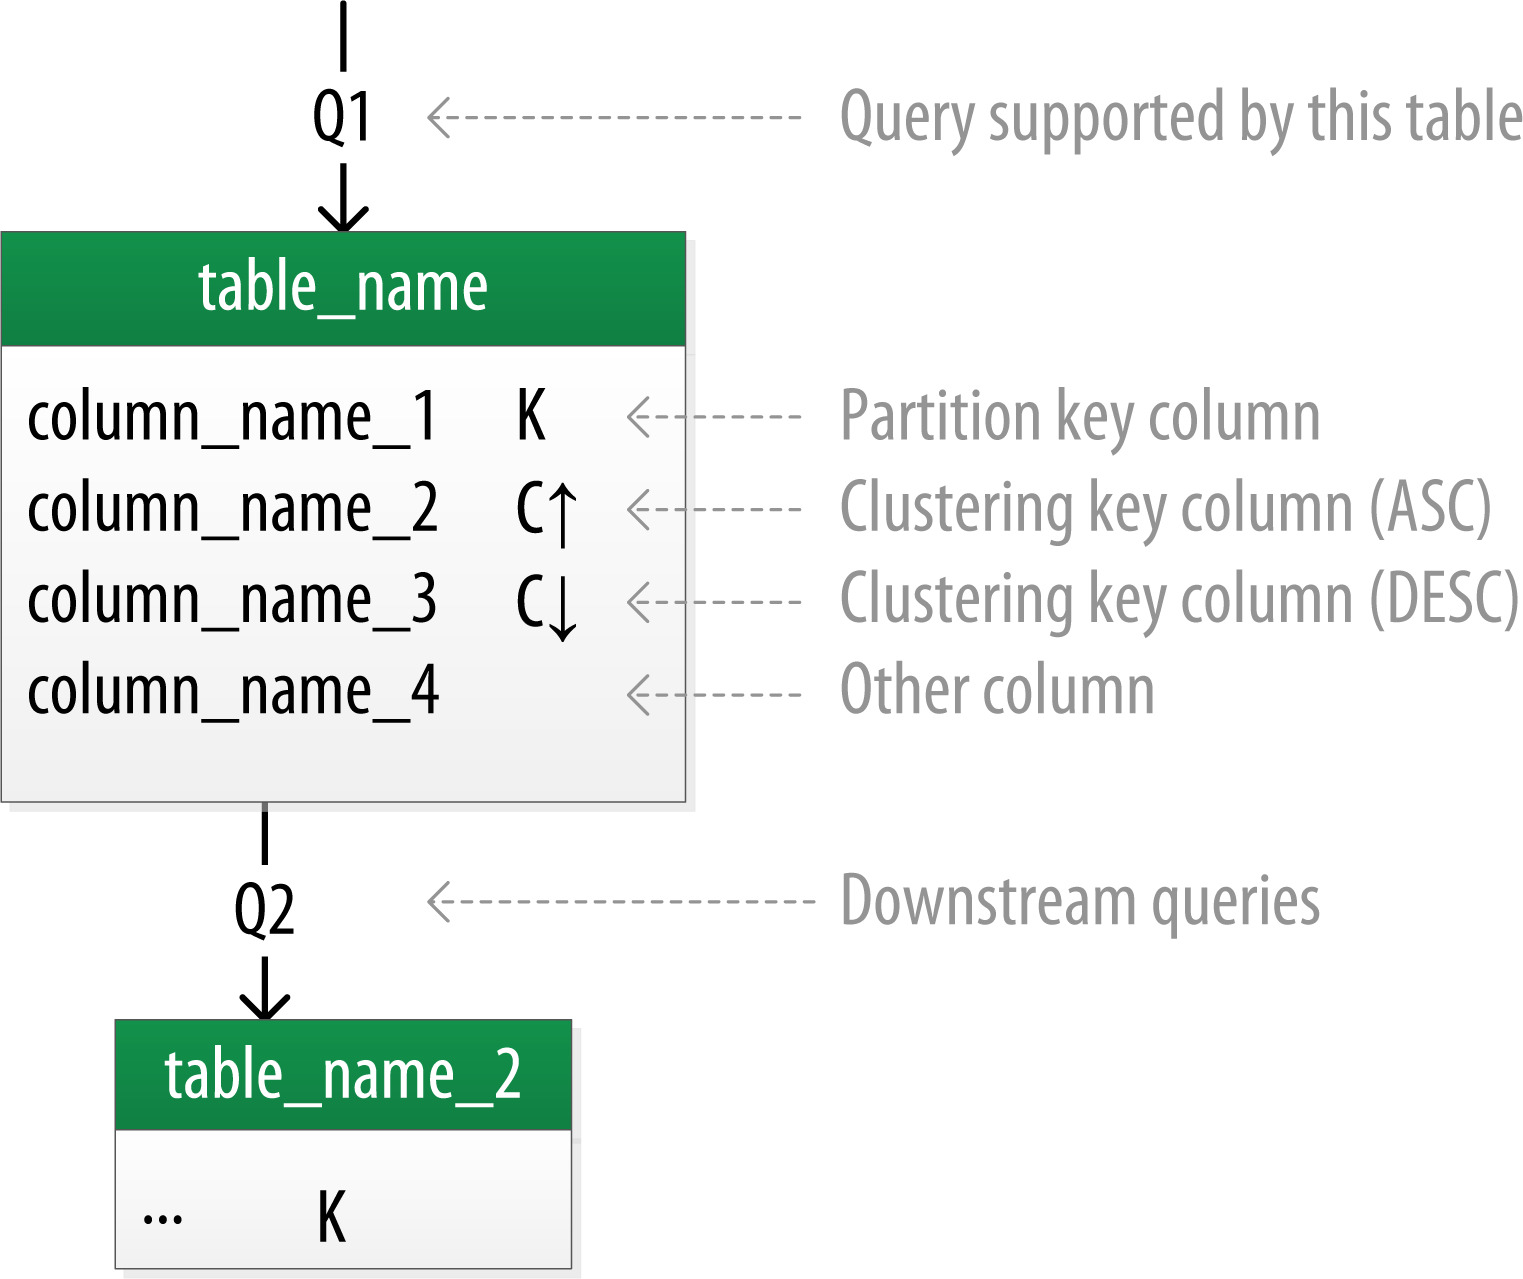
\includegraphics[width=0.75\columnwidth]{img/model_example_primary_key.jpeg}
    \caption{Model and denormalize tables to fit queries \autocite{cassandra_oreilly}}
    \label{fig:cassandra:chebotko}
\end{figure}

\section{Using the Cassandra Query Language} \label{sec:cassandra:cql} % How to use CQL
This section will give a short overview of how to interact with a Cassandra database using \gls{cql}, which is mainly inspired by \gls{sql} \autocite{cqlAlexMeng, newInCQL3, cassandra3cqldocCreateKeystore}.

\subsection {Creating a keyspace}
This similarity becomes clear by looking at how the creation of a keyspace is performed:
\begin{verbatim}
/* Create a new keyspace in CQL */
CREATE KEYSPACE data WITH replication =
    {'class': 'SimpleStrategy', 'replication_factor': 3};

/* Create a new database in SQL */
CREATE DATABASE data;
\end{verbatim}

Hereby the only difference is that instead of creating a database, a keyspace is created and it is possible to specify which replication parameters should be used. What these parameter mean and how they should be used is explained later in section~\ref{sec:CassandraClusterArchitecture} \autocite{cqlAlexMeng}.

\subsection{Creating a table}
After creating a keyspace a table has to be created in order to hold the data. As a database is always part of a keyspace it is either necessary to specify the keyspace in every query or to simple scope every subsequent query into a given keyspace by using the USE query \autocite{cassandra3cqldocUse}:
\begin{verbatim}
USE data;
\end{verbatim}

Using this keyspace a table can be created using the same syntax as in \gls{sql} \autocite{cqlAlexMeng, newInCQL3, cassandra3cqldocCreateTable}:
\begin{verbatim}
CREATE TABLE groups (
   group_name varchar,
   group_location varchar,
   added_date date,
   username varchar,
   PRIMARY KEY (...)
);
\end{verbatim}

Hereby the only difference is how the primary key can be specified:

\begin{figure}[ht]
    \centering
\begin{verbatim}
      partition key       clustering key  clustering key
       |       |                |            |
((groupname, group_location), added_date, username)
\end{verbatim}
    \caption{Parts of a primary key specification in \gls{cql} \autocite{cqlPrimaryKeyDefinition}}
    \label{fig:cassandra:primaryKeyDefinition}
\end{figure}

The first part of the definition will always be the partition key. If it is a compound of several columns they need to be surrounded by parentheses and separated by comma in order to state that they as a whole form the partition key. If necessary the partition key can be followed by several clustering keys. Keep in mind that the data will be ordered first by the first clustering key, after that by the second and so on. This means that an \texttt{ORDER BY} has to first be called on the first clustering key and a second ordering can be done on the subsequent one. It will not be possible to only order by the second or other subsequent clustering keys when not ordering by the first. Any other non-primary key column cannot be used for ordering \autocite{cqlPrimaryKeyDefinition, cassandra3cqldocCreateTable}.

\subsection{Interacting with data}
In order to manipulate Cassandra only provides three possible methods \autocite{cassandra_paper}:
\begin{itemize}
    \item insert(table, key, rowMutation)
    \item get(table, key, columnName)
    \item delete(table, key, columnName)
\end{itemize}
All having in common that the entire primary key has to be specified in order to interact with the data. The only exception hereby is the getting of data where only the partition key has to be specified.

Important to note is that there is no interaction to update a data entry. The reason for that is that as Cassandra is optimized for high write throughput is is very costly to read any data before writing. This means that the update and insert known from \gls{sql} will perform the same action on the data \autocite{cqlAlexMeng, newInCQL3}:
\begin{verbatim}
/* Inserting Data */
INSERT INTO Person (lastname, name, email)
  VALUES ('Doe', 'Jane', 'jane@example.com');

/* Updating Data */
UPDATE Person SET email = 'jane@example.com'
  WHERE lastname='Doe' AND name = 'Jane';
\end{verbatim}

As getting and deleting data is also similar to \gls{sql} there is no need to go into it any further in this section \autocite{cqlAlexMeng, cassandra3cqldocSelect}:
\begin{verbatim}
/* Selecting Data */
SELECT * FROM Person
  WHERE lastname='Doe' AND name = 'Jane';
/* Deleting Data */
DELETE FROM Person
  WHERE lastname='Doe' AND name = 'Jane';
\end{verbatim}

\section{Local reads and writes}
In order to perform the requested changed to the data they have to be written into the database. This section will take a look into how the changes will be written on a single node not taken into account the cluster.

\begin{figure}[ht]
    \centering
    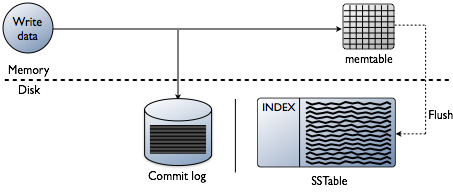
\includegraphics[width=0.75\textwidth]{img/cassandra_local_write.png}
    \caption{Writing data to Cassandra node \autocite{datastaxWriteData}}
    \label{fig:cassandra:writeData}
\end{figure}
In figure~\ref{fig:cassandra:writeData} it can be seen that the write process to Cassandra involves three steps:
\begin{enumerate}
\item \textbf{Write to journal} Hereby the query is simple append to the journal on the disk, making it persistent even if the node goes down. As this action is a simple append it is very fast and leaves the data in a temporal order in the journal.
\item \textbf{Write to memtable} After writing to the journal the change is performed in the memtable putting the data into a Sorted String Table (SSTable). This form is the same form in which the data will be written on disk. Here it is important that only the required data is written if there are any columns not specified it will not be written to the memtable. In contrast to writing \texttt{NULL} to a column which will delete it by setting a tombstone on it (See Appendix \ref{appendix:cassandra:queryExample}).
\item \textbf{Flush to disk when memtable is too big} This allows to simply flush the data and some metadata to the disk when it gets to big for the memory to hold it. Hereby a new data file is created, not touching any of the previously written files, making this action also quite fast as no lookups have to be performed.
\item \textbf{Compacting written datafiles} As writing to disk is only an append and will create a new datafile for every flush, the whole database will be scattered over multiple files with redundant data if entries were written after flushing them to disk. In order to merge these files it is possible to compact the files into one resulting in faster reads later \autocite{cassandraCompactTool}.
\end{enumerate}

After writing the data it also can be read again as shown by figure~\ref{fig:cassandra:readData}:

\begin{figure}[ht]
    \centering
    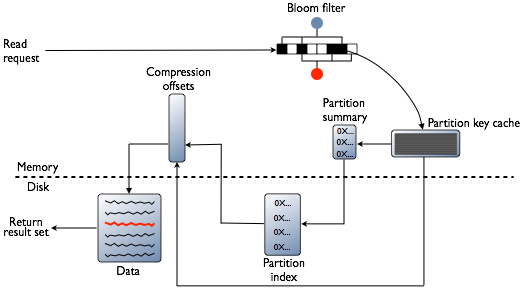
\includegraphics[width=0.75\textwidth]{img/cassandra_local_read.png}
    \caption{Reading data from Cassandra node \autocite{datastaxReadData}}
    \label{fig:cassandra:readData}
\end{figure}
\begin{enumerate}
    \item \textbf{Check caches} First the last query cache will be checked. Returning the data right away if it was requested in the near past.
    \item \textbf{Check memtable} If not found in the caches the memtable will be checked whether it has the most recent activities on the requested data.
    \item \textbf{Find SSTable and location} If no entry was found in the memtable the data on disk will be checked by firstly determining in which memtable dump the dataset will be and then retrieving it from there. For a detailed overview of this take a look at figure \ref{fig:cassandra:readData}
    \item \textbf{Merge with memtable} If it was necessary to retrieve the data from disk the data will be written to the memtable to allow later queries on the same data to succeed earlier.
\end{enumerate}

\section{Cluster Architecture}\label{sec:CassandraClusterArchitecture}  % How the cluster works
Which node has a certain piece of data is not determined by a master server. Any node has the ability to determine where a particular piece of data is or must be stored just by hashing the partition key of a row. The result of that calculation is called a token. All nodes are placed somewhere on a \textit{token ring} (see figure~\ref{fig:cassandra:tokenring}) and store the data of the tokens they are assigned to.\autocite[2]{cassandra_paper} \autocite[209,210]{decandia2007dynamo}

\newcommand{\Ray}{3cm}
\begin{figure}[ht]
  \centering
  \begin{tikzpicture}
    % Nodes on the circles
    \node[circle,minimum width=2cm,minimum height=1cm,draw,name path=n1] (Node A) at (90:\Ray) {A};
    \node[circle,minimum width=2cm,minimum height=1cm,draw,name path=n2] (Node B) at (0:\Ray) {B};
    \node[circle,minimum width=2cm,minimum height=1cm,draw,name path=n3] (Node C) at (270:\Ray) {C};
    \node[circle,minimum width=2cm,minimum height=1cm,draw,name path=n4] (Node C) at (180:\Ray) {D};

    % Circle the nodes are placed on
    \path[name path=c] circle (\Ray);
    \path[name intersections={of=n1 and c,name=i1},
          name intersections={of=n2 and c,name=i2},
          name intersections={of=n3 and c,name=i3},
          name intersections={of=n4 and c,name=i4}
         ];

    % Arrows between the nodes
    \begin{scope}
      \pgfsetarrowsend{Stealth[scale=1.5]}

      \pgfpathmoveto{\pgfpointanchor{i1-2}{center}}
      \pgfpatharcto{\Ray}{\Ray}{0}{0}{0}{\pgfpointanchor{i2-1}{center}}
      \pgfusepath{draw}

      \pgfpathmoveto{\pgfpointanchor{i2-2}{center}}
      \pgfpatharcto{\Ray}{\Ray}{0}{0}{0}{\pgfpointanchor{i3-1}{center}}
      \pgfusepath{draw}

      \pgfpathmoveto{\pgfpointanchor{i3-2}{center}}
      \pgfpatharcto{\Ray}{\Ray}{0}{0}{0}{\pgfpointanchor{i4-2}{center}}
      \pgfusepath{draw}

      \pgfpathmoveto{\pgfpointanchor{i4-1}{center}}
      \pgfpatharcto{\Ray}{\Ray}{0}{0}{0}{\pgfpointanchor{i1-1}{center}}
      \pgfusepath{draw}
    \end{scope}

    % Labels on arrows
    \node[fill=white] at (45:\Ray) {0 to 63};
    \node[fill=white] at (135:\Ray) {64 to 127};
    \node[fill=white] at (225:\Ray) {128 to 191};
    \node[fill=white] at (315:\Ray) {192 to 255};
  \end{tikzpicture}
  \caption{Token Ring}
  \label{fig:cassandra:tokenring}
\end{figure}

The tokens from the node's location to the next node belong to it. That means if the hashing of a partition key results in a token between 0 and 63 the data will be written to or read from node A. Keep in mind: This doesn't however mean that this node is \textit{in control} of that data - when replication is configured all replicas are equal. The node with that token is just the starting point to determine the first of the replicas.

\paragraph{Replication} To ensure that all data continues to be available even if some nodes go down Cassandra replicates the data in the cluster. Replication can be defined for each keyspace when it is created. There is a simple strategy and a network topology aware strategy. \autocite{datastax_replication} \\
The \texttt{SimpleStrategy} places the $n$ replicas of a piece of data on the next $n-1$ nodes\footnote{The first node that holds the data also counts as a replica.} located clockwise on the ring after the node with the token. \autocite[3]{cassandra_paper} \\
The \texttt{NetworkTopologyStrategy} strategy tries to be smart about the physical placement of replicas. It needs to be taught about in which datacenter and rack the nodes are located. To avoid losing data when an entire rack or datacenter fails this strategy prefers to spread it out.
It is recommended to use this strategy in production, unless all nodes are in a single rack, where both strategies are equivalent.

\paragraph{Rebalancing}

When a new node is added or a node is removed it is likely that the distribution of nodes on the ring becomes imbalanced. When the ring is imbalanced nodes are responsible for different amounts of data and experience different amounts of load. Since nodes are recommended to be of the same performance level\footnote{Or be balanced by dividing them up into virtual nodes according to performance} this is not optimal. Some nodes are overloaded and others underutilized.
To balance the ring the nodes are moved to equidistant positions on the ring. When this happens data is bound to be assigned to a new owner node - that data will be moved. \autocite{datastax_balancing}
The hash function used to transform partition key into is a so called \textit{consistent hash function}. The difference from a regular (cryptographically secure) hash function is that the output wraps around and thus can be represented as a ring. It also has the property that it minimizes the amount of shifting data that is necessary when a node is added or removed. \autocite{karger1997consistent}

Figure~\ref{fig:cassandra:rebalancing} visualizes an imbalanced ring and how the green nodes can be repositioned.


\begin{figure}[ht]
  \centering
  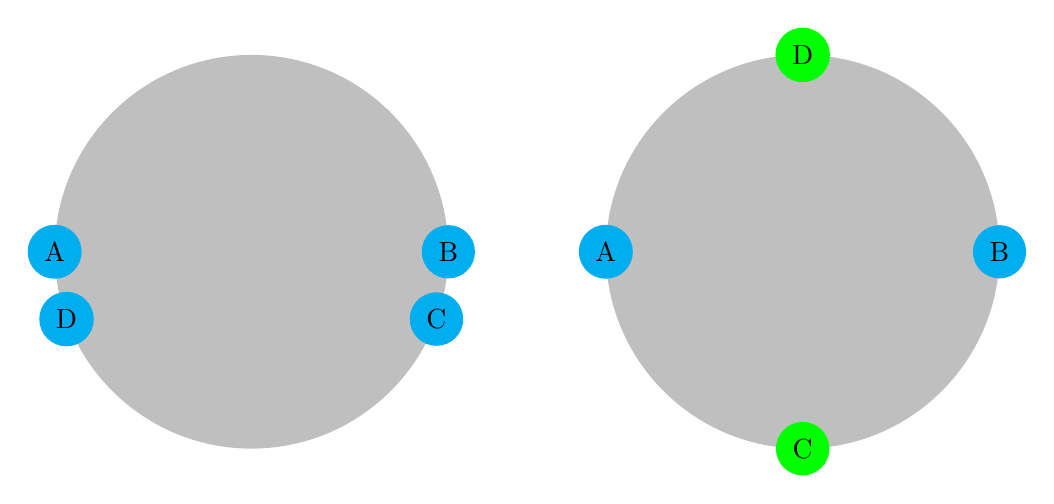
\begin{tikzpicture}
    % Circle
    \fill[fill=black!25] (2.5, 0) arc (0:360:2.5);
    \node[circle,fill=cyan] at (180:2.5) {A};
    \node[circle,fill=cyan] at (0:2.5) {B};
    \node[circle,fill=cyan] at (-20:2.5) {C};
    \node[circle,fill=cyan] at (200:2.5) {D};

    % Legend
    \begin{scope}[shift={(7,0)}]
      \fill[fill=black!25] (2.5, 0) arc (0:360:2.5);
      \node[circle,fill=cyan] at (180:2.5) {A};
      \node[circle,fill=cyan] at (0:2.5) {B};
      \node[circle,fill=green] at (270:2.5) {C};
      \node[circle,fill=green] at (90:2.5) {D};
    \end{scope}
  \end{tikzpicture}
  \caption{Rebalancing}
  \label{fig:cassandra:rebalancing}
\end{figure}

Nodes A and B can stay at their location, C and D are repositioned. C is moved further along the ring in a clockwise direction. It gives much of the data it was previously responsible to B and takes all of D's data. D is moved past A and takes approximately half of its data.

\paragraph{Virtual Nodes}

By default each node is placed on the ring just once, when using virtual nodes they each can be placed on the node multiple times. This brings four advantages: \autocite{datastax_vnodes, yelp_balancing}

\begin{itemize}
  \item Nodes can occupy a specified proportion of the ring
  \item Tokens are automatically calculated and assigned to nodes $rightarrow$ No manual rebalancing
  \item Data hotspots on the ring are handled my multiple nodes
  \item Rebuilding of replacements is faster
\end{itemize}

1. When nodes have different processing capabilities and disk space that performance difference should be taken into account so that all nodes receive load which is proportional to their performance. With virtual nodes enabled a node can be assigned any number of tokens. Not the absolute number of tokens of an individual node is relevant it only has an effect on how much of the ring it occupies on relation to the others.  \\
2. Without using virtual nodes the tokens for each node have to be calculated manually and assigned to each node. Cassandra also automatically rebalances the ring whenever a new node joins or a node leaves. \\
3. When data partitioning was done poorly or the data happens to cluster around a particular token range the node responsible for that data receives disproportionately much load. Virtual nodes remedy that because they not only make the individual partitions smaller but they also make any single note responsible for multiple areas on the ring. \\
4. When a node goes down and a replacement is brought up. This replacement needs the data of the node it replaced. If the replication factor is three it needs data from three different partitions. Without virtual nodes this can come from up to $3\cdot(3-1)=6$ different replicas. When using virtual nodes the partitions the same amount of data is spread across more nodes and thus the replication can transfer data from more nodes at once. If each node is split into $k$ virtual nodes it can replicate from $k$ times more replicas.

See figure~\ref{fig:cassandra:vnodes} for a visualization.

\begin{figure}[ht]
  \centering
  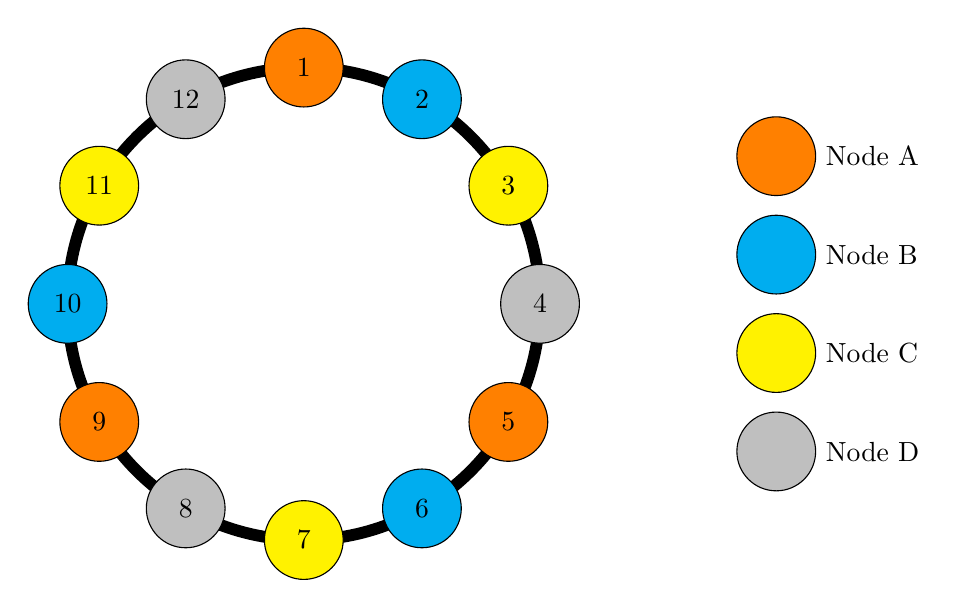
\begin{tikzpicture}
    % Circle
    \draw[line width=1.5mm] (\Ray, 0) arc (0:360:\Ray);

    % Nodes on the circle
    \foreach \x [count=\p] in {0,...,2} {
      \node[circle,draw,minimum size=1cm,fill=orange] at (90-\x*120-0*30:\Ray)
        {\pgfmathparse{1+4*\x}\pgfmathprintnumber{\pgfmathresult}};
      \node[circle,draw,minimum size=1cm,fill=cyan] at (90-\x*120-1*30:\Ray)
        {\pgfmathparse{2+4*\x}\pgfmathprintnumber{\pgfmathresult}};
      \node[circle,draw,minimum size=1cm,fill=yellow] at (90-\x*120-2*30:\Ray)
        {\pgfmathparse{3+4*\x}\pgfmathprintnumber{\pgfmathresult}};
      \node[circle,draw,minimum size=1cm,fill=black!25] at (90-\x*120-3*30:\Ray)
        {\pgfmathparse{4+4*\x}\pgfmathprintnumber{\pgfmathresult}};
    };

    \node[circle,draw,minimum size=1cm,fill=orange,label=right:{Node A}] at (2*\Ray, 1.875) {};
    \node[circle,draw,minimum size=1cm,fill=cyan,label=right:{Node B}] at (2*\Ray, 0.625) {};
    \node[circle,draw,minimum size=1cm,fill=yellow,label=right:{Node C}] at (2*\Ray, -0.625) {};
    \node[circle,draw,minimum size=1cm,fill=black!25,label=right:{Node D}] at (2*\Ray, -1.875) {};
  \end{tikzpicture}
  \caption{Virtual Nodes}
  \label{fig:cassandra:vnodes}
\end{figure}

\subsection{Distributed writes and reads (CAP Theorem)} \label{subsec:cassandra:cap}

Cassandra has a masterless architecture; no single node controls any particular piece of data \autocite[5]{cassandra_paper}\footnote{Unless explicitly configured to do so}. A consequence is that a client can run queries against any node of the cluster. In practice the client determines, either by some heuristic of proximity/latency or a round-robin algorithm, which node to use.
For one query that particular node becomes the \textit{coordinator node}; it coordinates the execution and distribution of that query.
First it hashes the partition key of the data to obtain the token and finds the node responsible for it. By using the replication strategy it can find out which replicas are responsible for that data as well. \\
When executing a read query the coordinator asks all replicas\footnote{A replica is every node responsible for that piece of data - the one determined by hashing as well as the others determined by replication strategy.} for the data. When more than \texttt{CL.read} replicas have answered the client is given an answer. When the replicas don't agree on the value of the data the client is sent the newest copy. Once all answers have come in the replicas with outdated information are sent a message on how to update their data, this is called a \textit{read repair}. \autocite{cassandra_distributed_read} \\
When executing a write query the coordinator sends the write request to all responsible replicas. If a replica is not currently available the coordinator logs the request and retries it later when the replica is back up  - this is called a \textit{hinted handoff}\autocite[6,7]{cassandraInCAPtheorem}. After more than \texttt{Cl.write} replicas have responded that they successfully completed the write the client is given a successful response. \autocite{cassandra_distributed_write}

For an explanation of the consistency levels \texttt{CL.read} and \texttt{CL.write} see section~\ref{subsec:cassandra:cap}.

In short, the process looks like this:

\begin{enumerate}
  \item Client sends query to any node
  \item That node becomes coordinator
  \item Coordinator determines tokens by hashing
  \item Coordinator sends write or read requests to all replicas determined by replication strategy
  \item For writing
    \begin{enumerate}
      \item Return success to client when more than \texttt{CL.write} nodes have acknowledged
      \item Write \textit{hinted handoff} to log for nodes that are currently unavailable
    \end{enumerate}
  \addtocounter{enumi}{-1}  % Both writing and reading should have the same number
  \item For reading
    \begin{enumerate}
      \item Return newest response when more than \texttt{CL.read} nodes have responed
      \item Send \texttt{read\_repair} to nodes with outdated data
    \end{enumerate}
\end{enumerate}

This process is also illustrated by figure~\ref{fig:cassandra:replication}.
The client queries node 4 which becomes the coordinator and then itself queries all replicas (1, 8 and 11).
When node 1 answers the default consistency level of \texttt{ONE} is satisfied and an answer is returned to the client.

\begin{figure}[ht]
  \centering
  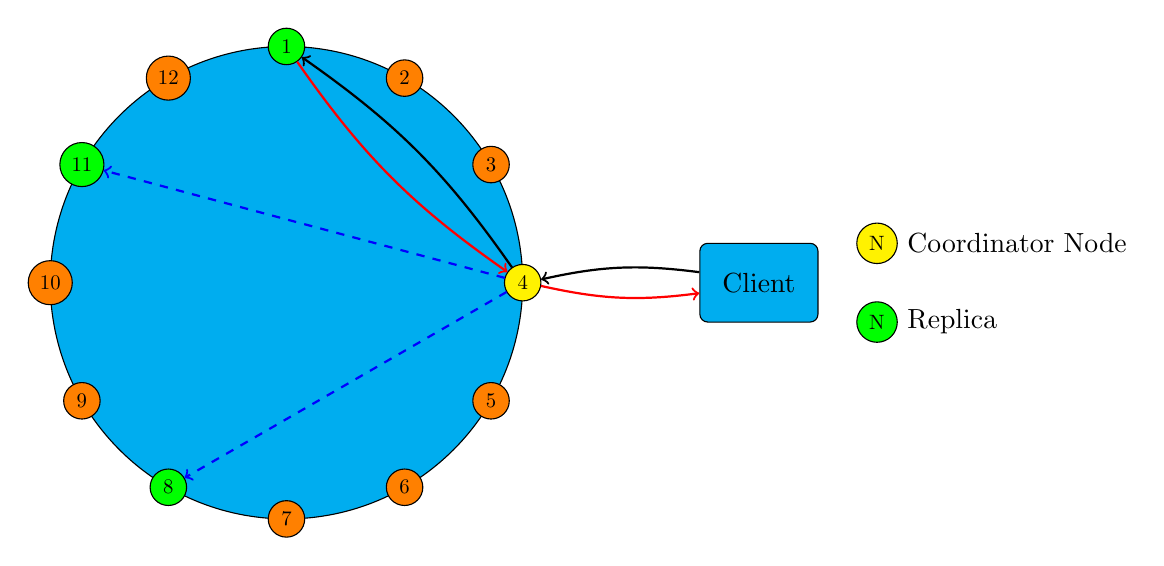
\begin{tikzpicture}
    % Circle
    \filldraw[fill=cyan] (\Ray, 0) arc (0:360:\Ray);

    % Nodes on the circle
    \foreach \x [count=\p] in {0,...,11} {
      \def\nodeColor{orange}
      \ifnum \p=1
        \def\nodeColor{green}
      \fi
      \ifnum \p=8
        \def\nodeColor{green}
      \fi
      \ifnum \p=11
        \def\nodeColor{green}
      \fi
      \ifnum \p=4
        \def\nodeColor{yellow}
      \fi
      \node[circle,draw,scale=0.75,fill=\nodeColor] (\p) at (90-\x*30:\Ray) {\p};
    };

    % Arrows between the nodes
    \draw [->,thick] (4) to[bend right=10] (1);
    \draw [<-,thick,draw=red] (4) to[bend left=10] (1);
    \draw [->,thick, dashed, blue] (4) -- (11);
    \draw [->,thick, dashed, blue] (4) -- (8);

    % Client plus its arrows
    \node[fill=cyan,draw,minimum width=1.5cm,minimum height=1cm,rounded corners=.1cm] (Client) at (2*\Ray, 0) {Client};
    \draw [->,thick,draw=red] (4) to[bend right=10] (Client);
    \draw [<-,thick] (4) to[bend left=10] (Client);

    % Legend
    \node[circle,draw,scale=0.75,fill=yellow,label=right:{Coordinator Node}] (coordinatorLegend) at (2.5*\Ray, 0.5) {N};
    \node[circle,draw,scale=0.75,fill=green,label=right:{Replica}] (replicaLegend) at (2.5*\Ray, -0.5) {N};
  \end{tikzpicture}
  \caption{Replication}
  \label{fig:cassandra:replication}
\end{figure}

\paragraph{Tuning Consistency} By default writes and reads need to be acknowledged by only a single replica. Usually data is configured to be replicated over multiple nodes. The result is that queries to Cassandra are highly available - any particular node can fail and the request will receive a successful response. This comes at the cost that not all replicas always have the same data - a lack of consistency. \\
Because different applications have different requirements of availability and consistency Cassandra offers several parameters to adjust its alignment on that spectrum.

One of those is the consistency level. As previously mentioned in this section it determines how many nodes have to acknowledge a request until enough nodes have acknowledged completion. Consistency level for reading and writing are abbreviated as \texttt{CL.read} and \texttt{CL.write} respectively.

Cassandra offers these, but not limited to these, options. \autocite{datastax_consistency_level}

\begin{itemize}
  \item \texttt{ALL} replicas
  \item \texttt{QUORUM}: A majority of the replicas: half + 1
  \item \texttt{THREE} replicas
  \item \texttt{TWO} replicas
  \item \texttt{ONE} replicas (default)
  \item \texttt{ANY}: Only writing - At least one replica or a logged \textit{hinted handoff} if all are unavailable
\end{itemize}

In addition to these levels Cassandra also offers others that also take into account how nodes are distributed into different datacenters. \\
For each query, but usually an entire client session, the consistency level can be chosen.

The \texttt{ALL} level yields the highest consistency. Only when all replicas have responded the response is given to the client. That means either all were updated or all were asked for their current dataset. Thus there is no uncertainty about what the result is - all replicas must agree. The \texttt{ANY} consistency level is the least consistent. The data does not have to be fully written to any SSTable, memtable or even commit log of a replica - a simple \textit{hinted handoff} on the coordinator is enough. \autocite[6,7]{cassandraInCAPtheorem}

\paragraph{Replication Factor} Whenever creating a keyspace you have to configure its replication strategy. Whatever strategy you choose you have to determine how often you want a piece of data to be replicated. If you go with the lowest possible value of 1 the failure of any node will inevitably lead to data loss (read and write failures). Increasing the replication factor means that more nodes can fail while requests can still be properly responded to - this means increased availability. It will, however, also mean that the additional replicas can get out of sync, which lowers the consistency. \autocite[3]{cassandra_paper}

We see that by default Cassandra is highly available and only eventually consistent but it can be gradually tuned to being highly consistent but more prone to failure. \autocite[2,3]{cassandraInCAPtheorem}

\section{Setup and Configuration}  % Setup
Cassandra is designed to be run in a cluster of multiple machines. That has to be kept in mind, even when setting up a single instance. That single instance would form a single node cluster. This makes manual configuration unavoidable - every node needs to know how to join the cluster.
For the purpose of joining the cluster each node is configured with a list of \textit{seed nodes}. When starting up for the first time it asks those nodes about the state of the ring and the new node is assigned a place on the ring. After joining the cluster is complete and the distinction of \textit{seed nodes} is no longer relevant - all nodes are equally important.
When a new node was added it is responsible for a chunk of the data the others were previously responsible for. They do not remove that, now unnecessary, data on their own - to do so run \texttt{nodetool cleanup} on each of the old nodes.

A simple but sufficient\footnote{The other settings can be left at their defaults.} configuration of the first node would look like shown in listing~\ref{lst:cassandra:first_node_config}. \autocite{cassandra_config}

\begin{listing}[ht]
  \begin{minted}{yaml}
# Open socket on this address
listen_address: "192.168.0.2"
# Tell other nodes its reachable on this address
broadcast_address: "3.14.1.59"

seed_provider:
  - class_name: org.apache.cassandra.locator.SimpleSeedProvider
    parameters:
      - seeds "3.14.1.59"

# Enable client communication
start_native_transport: true
  \end{minted}
  \caption{Configuration of first node}
  \label{lst:cassandra:first_node_config}
\end{listing}

For the masterless cluster to function all nodes need to be able to reach all other nodes. This is trivial if all are in the same subnet of the network. Then they can just reach each other by their IP addresses.
When they are in different subnets however they each have a private (local to their subnet) and public (inter subnet) address. This is very often the case in public cloud offerings. There are just not enough addresses available to give every node a public one.
Cassandra needs to know two things:
1. On what address to listen for oncoming TCP connections. That's what \texttt{listen\_address} is for. This is the local/private address.
2. What address to tell other nodes it's reachable under. This is set by \texttt{broadcast\_address} and it is the public address that all other nodes must be able to reach.
Therefore in a local network (with no address translation between the nodes) \texttt{listen\_address} and \texttt{broadcast\_address} are set to the same value.

In order to create a single cluster instance the node has to have its seed set to containing only its own address. Since it doesn't need to listen on a public or even private IP this should, in most cases, be \texttt{localhost}.
The first node of a cluster can be thought of as such a single instance node until others join.

In order for additional nodes to join the cluster configure them analogous to the first, changing the address values but keeping the seed list.
Upon starting them they will automatically communicate with the seed and join the cluster.

\paragraph{More configuration} Cassandra has many more parameters that we are not going to mention here. They can be used to adjust everything from performance tuning, architectural changes or increasing security.
To use virtual nodes explained in section~\ref{sec:CassandraClusterArchitecture} and give a node more than a single token the \texttt{num\_tokens} parameter can be used. \autocite{cassandra_config}
In its default configuration Cassandra claims a few gigabytes of memory. On dedicated Cassandra nodes you would probably want to increase it to fully utilize the hardware. However for testing purposes you do not want it to consume a big chunk of your memory. Our experience has shown that Cassandra does not like being given too little memory and is prone to crashing if that happens. To adjust how much memory Cassandra uses the \texttt{MAX\_HEAP\_SIZE} and \texttt{HEAP\_NEWSIZE} variables in \texttt{/etc/cassandra/casandra-env.sh} can bet set. \autocite[281]{cassandra_oreilly}

\paragraph{Setup Overview} Setting up a service in a cluster architecture can be daunting because it involves many different components that all need to interact with eachother. The following list gives an overview over the tasks that need to be done:

1. Acquire enough capable nodes. DataStax the main contributor to Cassandra recommends to use at least 3 nodes, 8 cores, 32GB \\  % TODO cite
2. Set up a network between the nodes so that each one has a unique IP address and every node can reach every other node.\footnote{Multiple nodes behind a single NATed public IP is not possible because Cassandra allows only configuration of the broadcast IP but not the port} \\
3. Adapt the configuration files like shown above \\
4. Open the necessary port in the firewall: TCP/7000 for node to node communication (\texttt{storage\_port}) and TCP/9042 for client to node communication (\texttt{native\_storage\_port}). \\
5. Start all seed nodes and once they're online start the other nodes. \\

When that's done and all nodes have fully joined the cluster you can interact with the cluster with the \texttt{nodetool} and \texttt{cqlsh} tools.

\iffalse
\paragraph{Security}
\begin{itemize}
  \item Use a firewall to not expose it to the public internet  % Basic due diligence
  \item Internode communication with TLS  % TLS is always good $\rightarrow$ Encryption, Authenticity
  \item Client $\leftrightarrow$ Node communication with TLS
  \item JMX management only on localhost and with auth
  \item Authentication with password
  \item Disable default role  % There are no users, only roles (good RBAC model)
  \item Use roles
\end{itemize}
\fi

\iffalse
\paragraph{Comparison to similar data stores}
\begin{tabular}{l|l}
  Name & Description \\
  \hline
  Amazon DynamoDB & Amazon makes the decisions for you \\
  % Original developers of DynamoDB created Cassandra
  % Easy but less tunable
  % MultiCloud, Partitions, Nodes, Consistency level, ...
  % Cassandra based off of DynamoDB
  Google BigTable & Based on GFS (CP), Managed by Google \\
  % Can be used with Cassandra like architecture (default)
  ScyllaDB & Cassandra rewrite with better performance \\
  % C++ and better handling of multiple requests
  % Not yet all features and not "battle tested"
  Apache HBase & Similar data model, master/slave $\rightarrow$ CP\\
\end{tabular}
\fi

\section{Summary and Conclusion}
    %- Summary, most important parts (results)
    %- Limitations => Future research
    %- All questions that came up ^
    %- Research Question: Answer
    %- Discussion
    %- Conclusion

This chapter gave an overview about what Cassandra is, when to use it and detailed insights on how to use it and its architecture. It has shown that Cassandra is a complex database system with unique benefits compared to other database systems. It solves a lot of problems that come with big data environments. Due to its uniqueness it has to be assessed very carefully whether Cassandra is a fit for a certain environment or not. Although it comes with major benefits and extra features, some expected features and base assumptions about a database system are different in Cassandra.
It could be seen, that it is a great fit for lots of fast writes environments but comes short in OLTP environments where traditional RDBMS databases shine.
During the work on this chapter and the learning phase about Cassandra, it showed how detail rich and complex the solutions this distributed database storage brings with is. To truly understand Cassandra in all its different settings, possibilities and to be able to setup, run and maintain a production ready big sized cluster, more reading is needed. Especially the fine details how a Cluster will react in certain distress situations should be fully understood and can be assessed further.
